\chapter{Proposition de modèle de machine learning}
\label{chap:proposition_modele}

Ce chapitre va explorer la création d'un modèle de machine learning de A à Z.

\localtableofcontents

\newpage

% -----------------------------------------------------------------------------
% -----------------------------------------------------------------------------
\section{Introduction}
La création d'un modèle de machine learning implique plusieurs phases. La Figure \ref{fig:ch3_resume_machine_learning_supervise} résume les principales étapes et servira de fil conducteur pour le chapitre.
\begin{figure}[H]
    \centering
    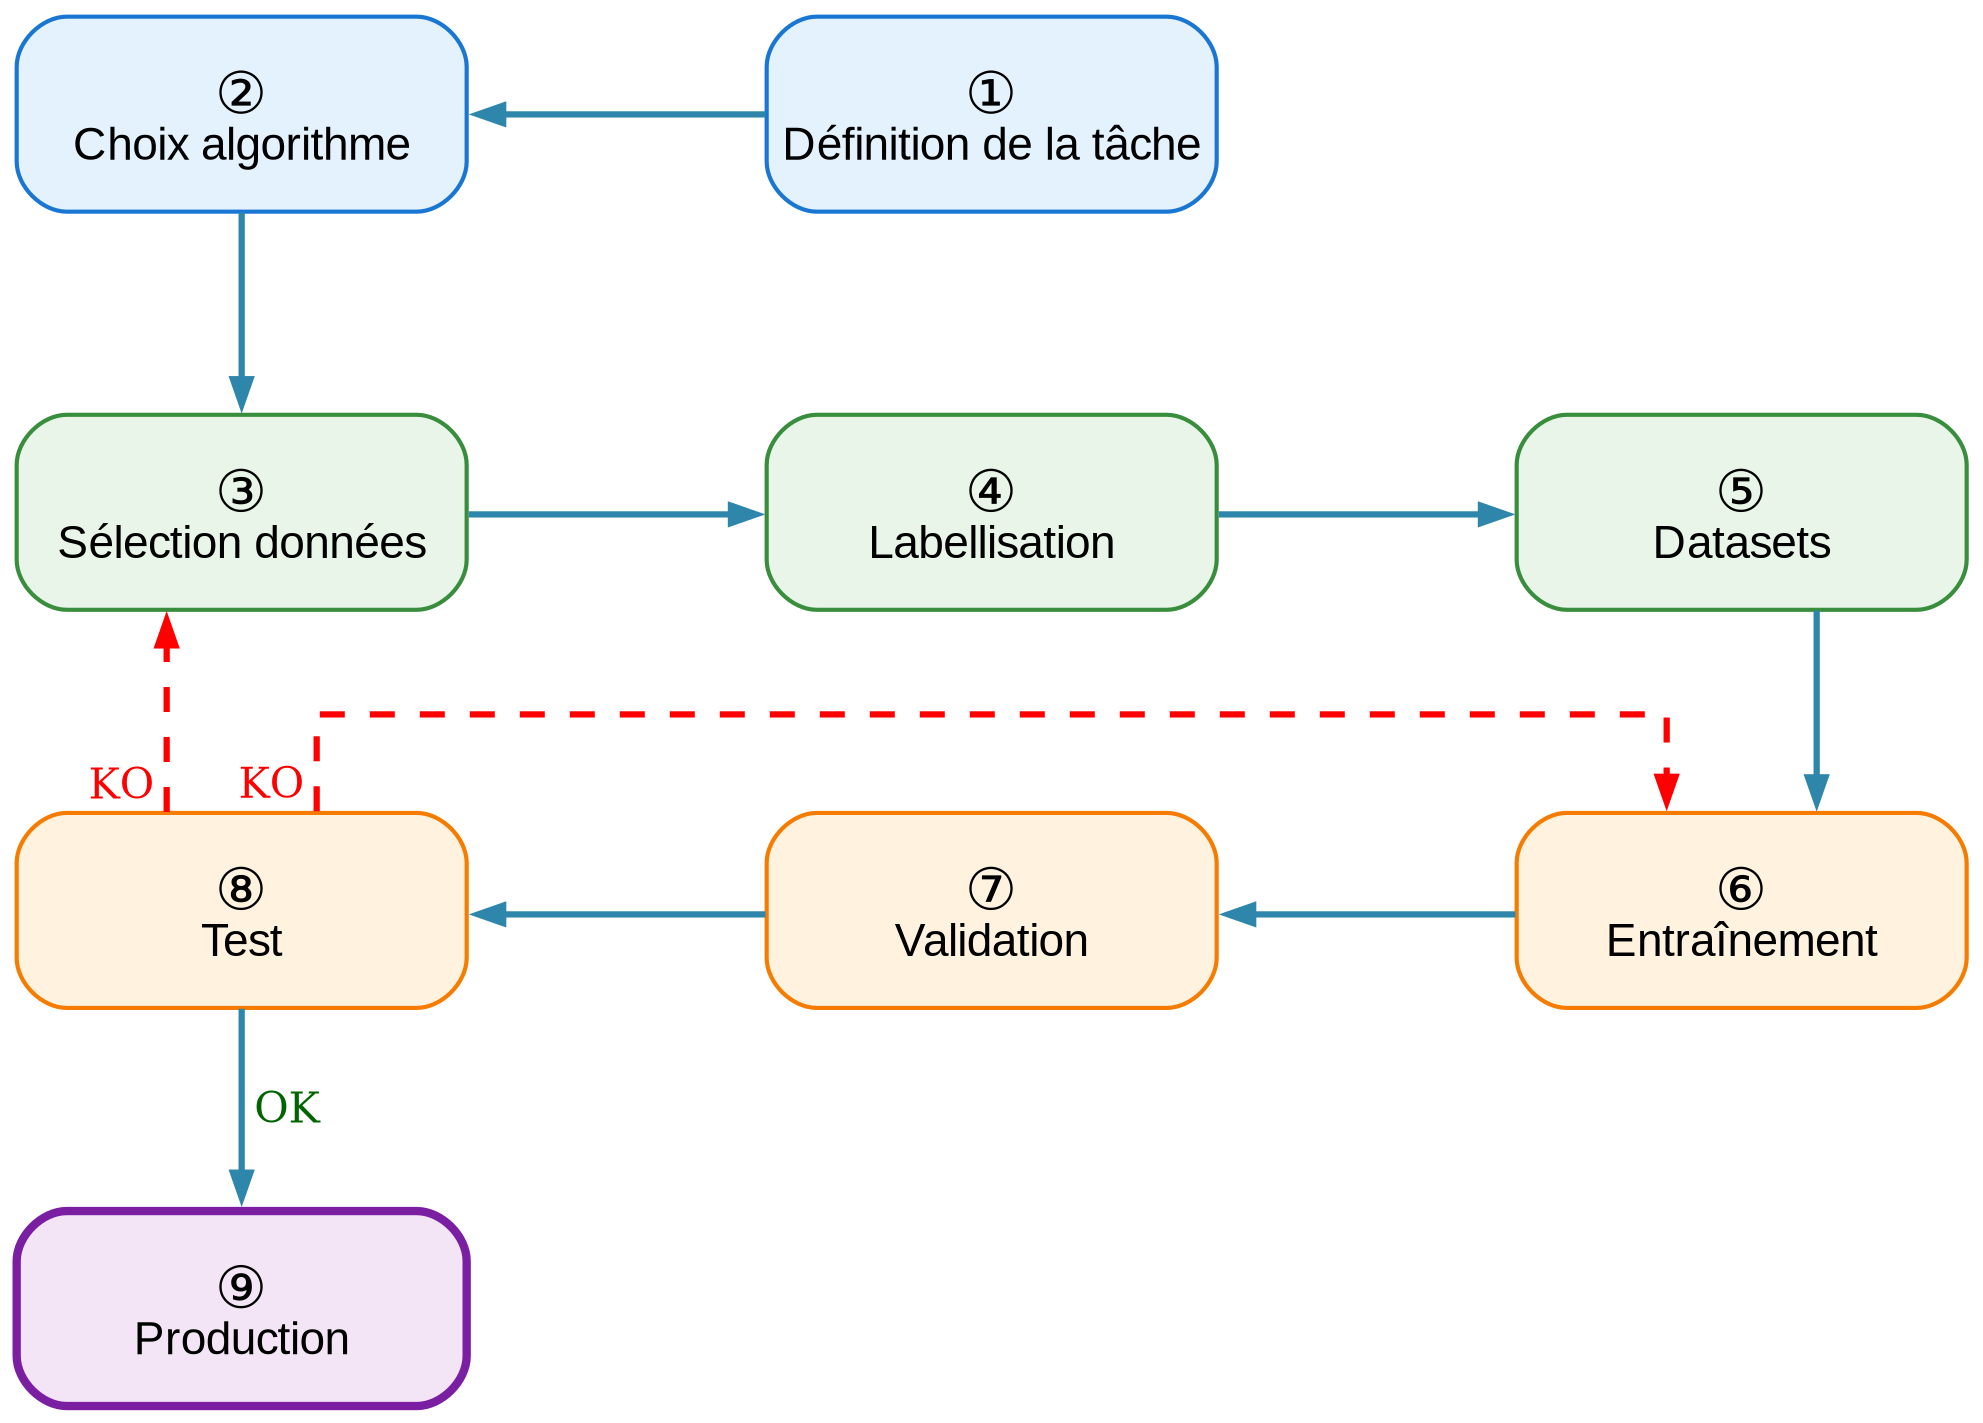
\includegraphics[width=1\linewidth]{03-tail/A1_fondamentaux_ML/A1_figures/A1_01_resume_machine_learning_supervise.png}
    \caption{Résumé de machine learning supervisé}
    \label{fig:ch3_resume_machine_learning_supervise}
\end{figure}
En premier il faut définir la tâche et choisir le bon algorithme. Ensuite selon les besoins en données, il faut créer un dataset pour entraîner le modèle. Finalement lorsque le modèle est suffisamment performant, il peut être utilisé en production.

L'Annexe \ref{chap:fondamentaux_ml} permet de se familiariser avec l'ensemble des termes et concepts de machine learning utilisés dans ce chapitre.

% -----------------------------------------------------------------------------
% -----------------------------------------------------------------------------
\section{Phase préparatoire}
Cette phase préparatoire intègre les 2 premières étapes de la Figure \ref{fig:ch3_resume_machine_learning_supervise}, c'est-à-dire la définition de la tâche à accomplir et le choix de l'algorithme.

\subsection{Tâche}
La tâche que ce modèle doit accomplir est d'identifier les espaces disponibles sur les toitures. Cette tâche est identique à celle de \acrshort{stdl} du chapitre \ref{subsec:stdl_analyse}, par contre l'approche utilisée va être différente.

\subsection{Algorithme}
Une fois la tâche définie, il faut déterminer une approche. \acrshort{stdl} avait exploré 3 approches différentes:
\begin{itemize}
    \item La classification des pans de toit
    \item La segmentation des données \gls{lidar}
    \item La segmentation d'images
\end{itemize}

Leur segmentation d'images est réalisée avec Segment Anything Model (SAM). SAM effectue de la segmentation instance et divise l'image en polygones mais n'assigne pas une classe aux objets. Les résultats doivent être post-traités pour identifier les espaces disponibles. Un autre point délicat est le temps de traitement important (12 minutes pour 25 bâtiments).

La segmentation sémantique est une autre option explorée par \citeauthor{castello_quantification_2021} (Section \ref{subsec:castello_quantification_2021}). Ils l'ont utilisé pour exactement la même tâche avec un dataset limité au centre ville de Genève. Les résultats obtenus avec un IoU supérieur a 0.60 sur leur dataset de test sont très encourageants.

La segmentation sémantique est le type d'algorithme retenu.

\section{Autres pistes explorées}
Plusieurs autres approches ont été explorées, le but initial étant d'éviter de devoir créer un dataset. La génération d'un dataset pour une tâche tel que la segmentation sémantique exige une grande quantité d'images annotées. La première approche est d'essayer de classifier les données géomatiques, la deuxième approche implique l'utilisation de segment-anything-model.

\subsection{Classification}
La première approche a été d'essayer un algorithme de classification avec les données géomatiques.

Une autre piste explorée est l'utilisation de segment-anything-model (SAM) pour 

\begin{figure}[H]
    \centering
    
    % Première ligne
    \begin{subfigure}[b]{0.48\textwidth}
        \centering
        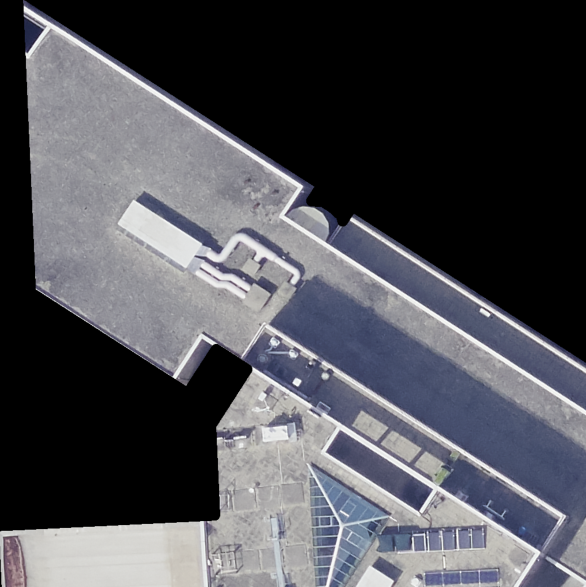
\includegraphics[width=\textwidth]{02-main/figures/ch3_essai_sam_01_image_original.png}
        \caption{Image d'exemple}
        \label{fig:ch3_essai_sam_01_image_original}
    \end{subfigure}
    \hfill
    \begin{subfigure}[b]{0.48\textwidth}
        \centering
        
\includegraphics[width=\textwidth]{02-main/figures/ch3_essai_sam_02_ROI.png}
        \caption{Zone d’intérêt (ROI)}
        \label{fig:ch3_essai_sam_02_ROI}
    \end{subfigure}
    
    \vspace{0.35cm} % Espace entre les lignes
    
    % Deuxième ligne
    \begin{subfigure}[b]{0.48\textwidth}
        \centering
        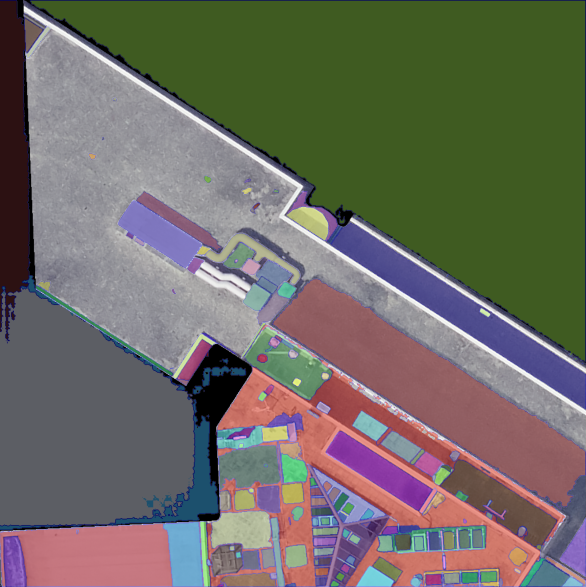
\includegraphics[width=\textwidth]{02-main/figures/ch3_essai_sam_03_200_masks.png}
        \caption{Polygones segmentés (200)}
        \label{fig:ch3_essai_sam_03_200_masks}
    \end{subfigure}
    \hfill
    \begin{subfigure}[b]{0.48\textwidth}
        \centering
        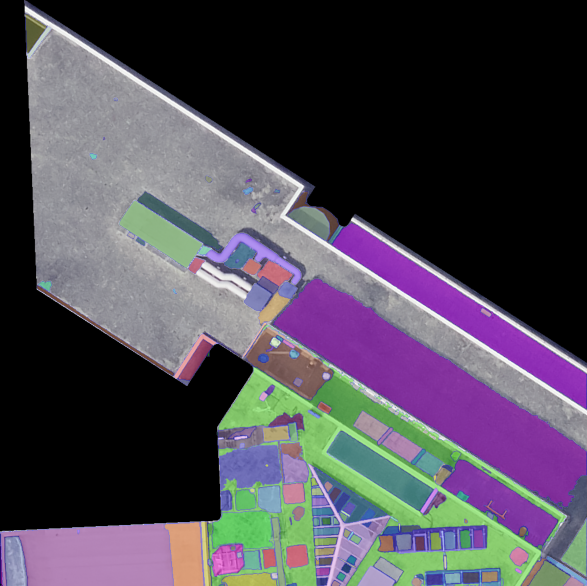
\includegraphics[width=\textwidth]{02-main/figures/ch3_essai_sam_04_194_filtered_masks.png}
        \caption{Polygone segmentés filtrés (194)}
        \label{fig:ch3_essai_sam_04_194_filtered_masks}
    \end{subfigure}

    \vspace{0.35cm} % Espace entre les lignes
    
    % Troisième ligne
    \begin{subfigure}[b]{0.48\textwidth}
        \centering
        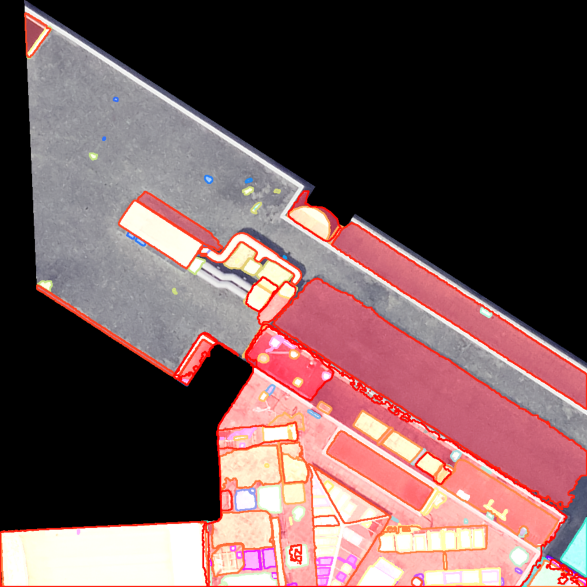
\includegraphics[width=\textwidth]{02-main/figures/ch3_essai_sam_05_filtered_masks_overlay.png}
        \caption{Mise en évidence des polygones filtrés}
        \label{fig:ch3_essai_sam_05_filtered_masks_overlay}
    \end{subfigure}
    \hfill
    \begin{subfigure}[b]{0.48\textwidth}
        \centering
        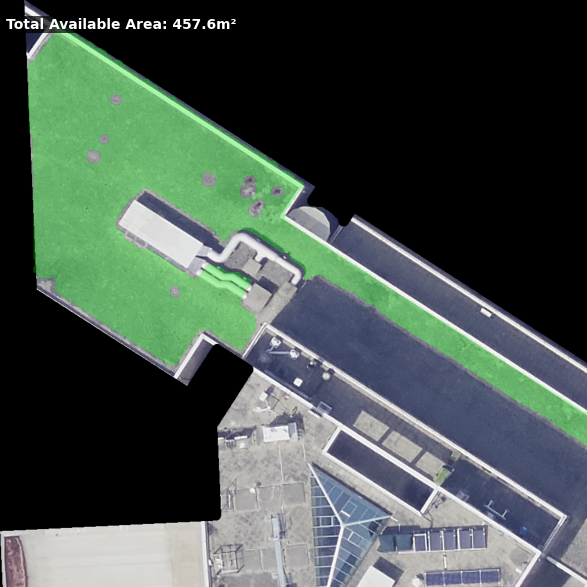
\includegraphics[width=\textwidth]{02-main/figures/ch3_essai_sam_06_une_zone_libre.png}
        \caption{Espace libre}
        \label{fig:ch3_essai_sam_06_une_zone_libre}
    \end{subfigure}

    \caption{Essai d'utilisation de SAM}
    \label{fig:essai_algo_sam}
\end{figure}








L'examen des datasets disponibles (Section \ref{sec:dataset_disponible}) révèle une carence majeure : seul le dataset RID propose des annotations pour l'identification des espaces libres sur toitures. Ce dataset présente toutefois des limitations importantes, avec des images concentrées sur un contexte architectural spécifique (rural allemand) et des performances dégradées lors des tests sur d'autres typologies de bâtiments, comme le démontrent les essais sur le milieu urbain bruxellois.

La création d'un dataset pour une tâche telle que la segmentation sémantique d'images est une tâche laborieuse et chronophage. La première section de chapitre va explorer certaines pistes envisagées qui n'ont finalement pas été retenues. Cette section permet de justifier la nécessité de créer un tel jeu de données annoté.

La deuxième section explore la création du dataset et finalement une troisième section va permettre de faire une synthèse en guise de conclusion de ce chapitre.

% -----------------------------------------------------------------------------
% -----------------------------------------------------------------------------
\section{Méthodologie}
Cette section détaille comment le dataset a été réalisé. Les étapes importantes sont l'obtention des données, le nettoyage, la préparation, la vérification et annotation des données.
\subsection{Données utilisées}
Les données utilisées proviennent de \acrshort{sitg}:
\begin{itemize}
    \item Données vectorielles
    \begin{itemize}
        \item Bâtiments hors-sol ``CAD\_BATIMENT\_HORSOL'' \cite{sitg_batiments_nodate}
        \item Toits des bâtiments ``CAD\_BATIMENTS\_HORSOL\_TOIT'' \cite{sitg_toits_nodate}
        \item Superstructures des toits des bâtiments ``CAD\_BATIMENT\_HORSOL\_TOIT\_SP'' \cite{sitg_superstructures_nodate}
        \item Communes genevoises ``CAD\_COMMUNE'' \cite{sitg_communes_nodate}
    \end{itemize}
    \item Données raster (images)
    \begin{itemize}
        \item Orthophotos 2019 \cite{sitg_orthophotos_nodate}
    \end{itemize}
\end{itemize}
\subsubsection{Données vectorielles}
Les données vectorielles sont en format GPKG \cite{noauthor_ogc_nodate}, ce format est assez commun dans le monde de la géomatique.
\todo[inline]{Ajouter ici le lien correct à l'annexe des données vectorielles}
\paragraph{Bâtiments hors-sol}
La couche vectorielle ``CAD\_BATIMENTS\_HORSOL'' recense tous les bâtiments du Canton de Genève qui sont bien ancrés au sol. Cette couche n'inclus pas les bâtiments qui sont sous-terrains. La Figure \ref{fig:dataset_methodo_01_batiment_horsol} permet d'observer ces polygones qui représentent les bâtiments en orange. Seulement le contour de la toiture est représenté.
\begin{figure}[H]
    \centering
    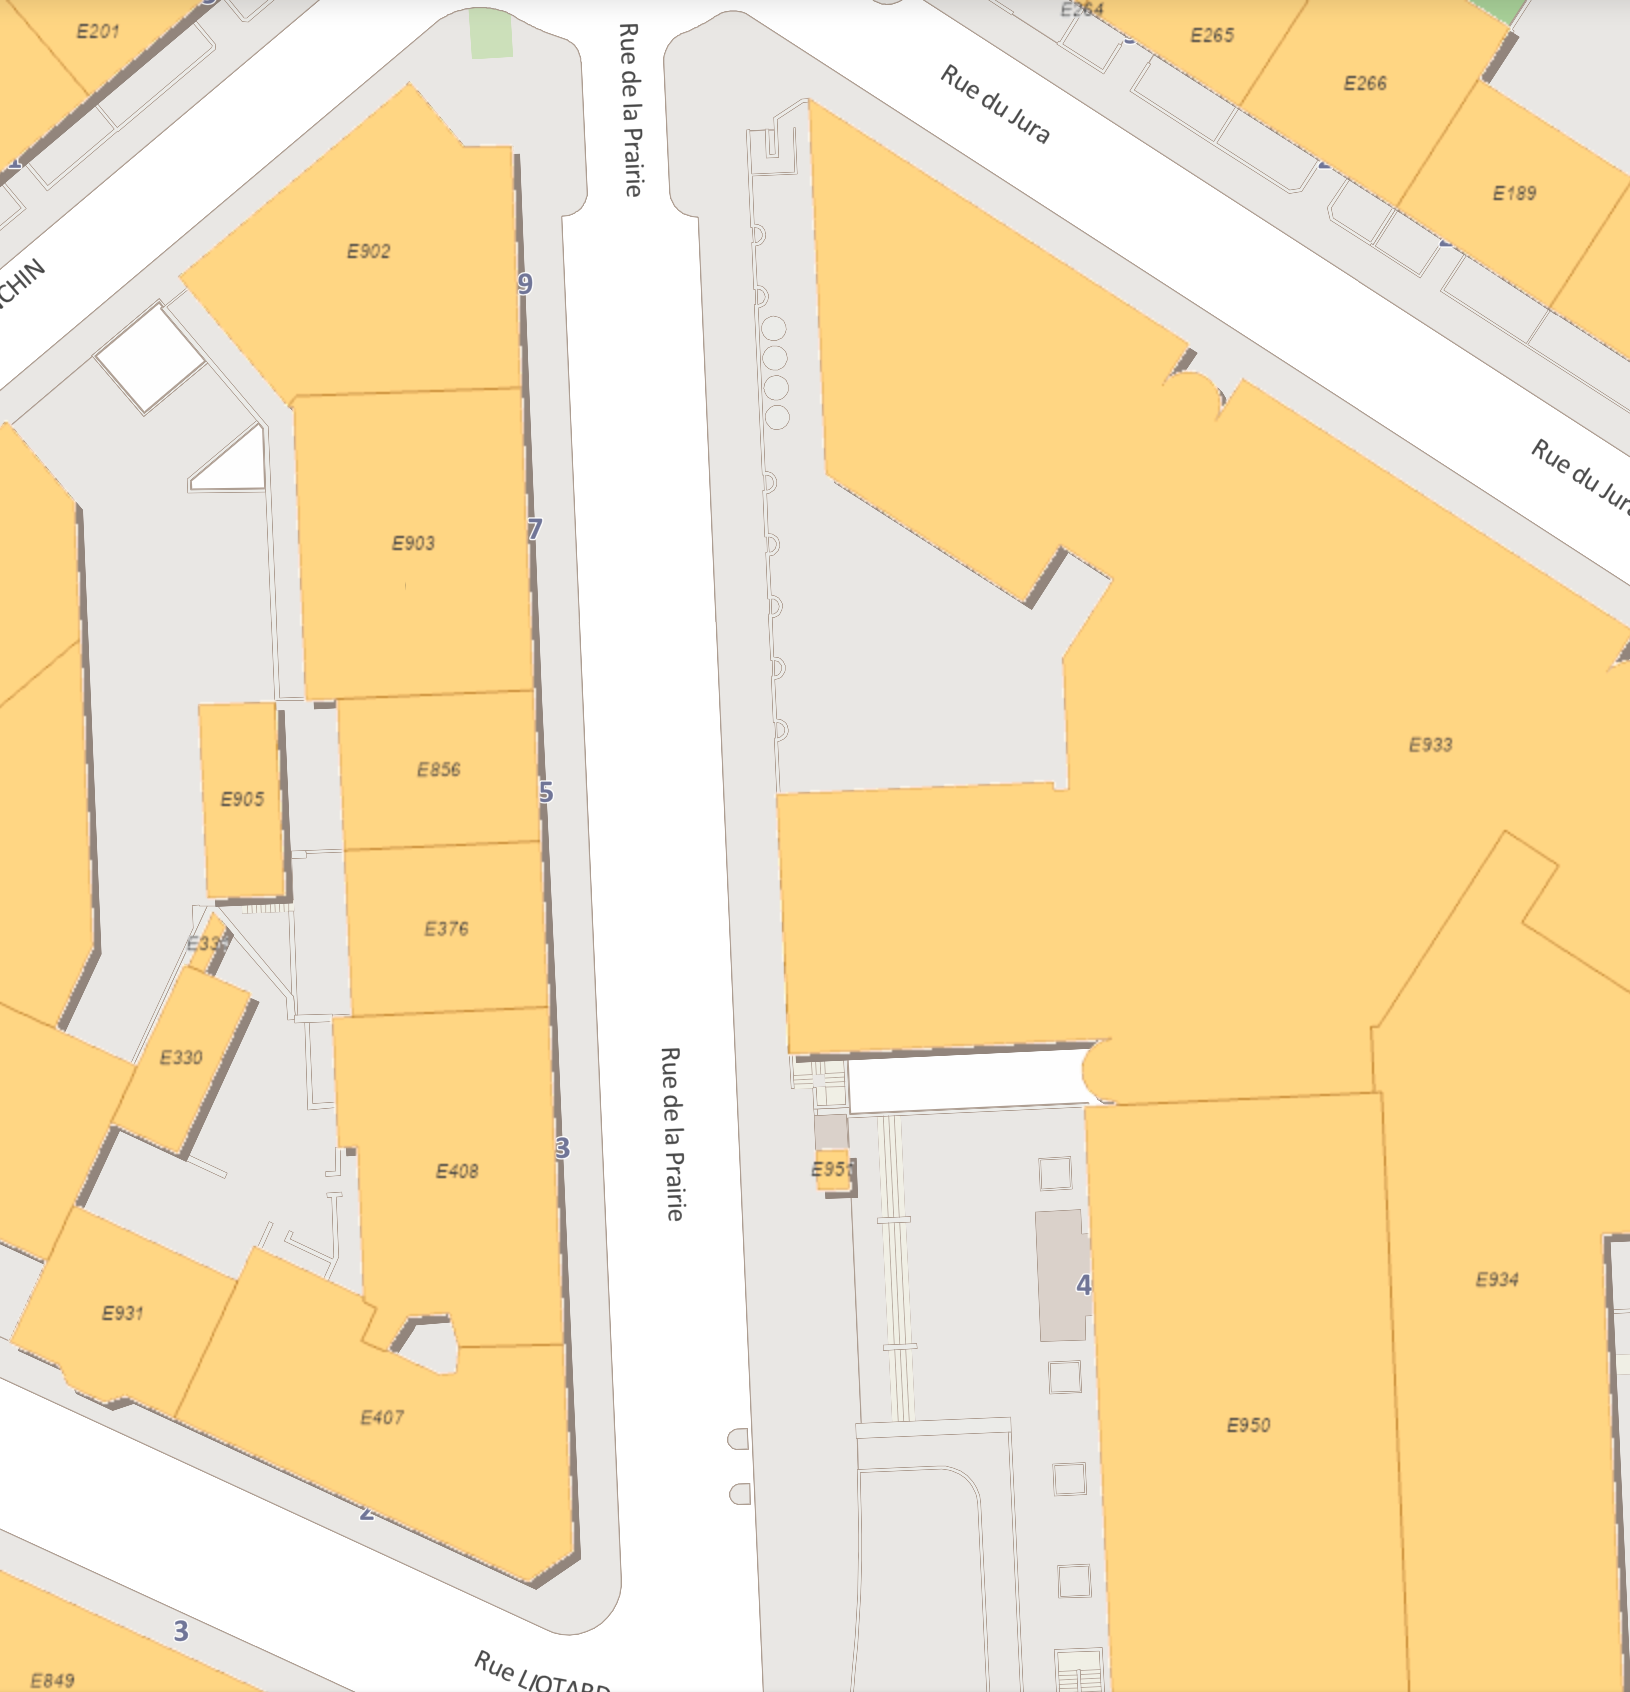
\includegraphics[width=1\linewidth]{02-main//figures/dataset_methodo_01_batiment_horsol.png}
    \caption{Couche vectorielle bâtiments hors-sol.}
    \label{fig:dataset_methodo_01_batiment_horsol}
\end{figure}
Cette couche vectorielle est enrichie de données tabulaires (Figure \ref{fig:dataset_methodo_02_batiment_horsol_donnees}) associées à chacun des polygones.
\begin{figure}[H]
    \centering
    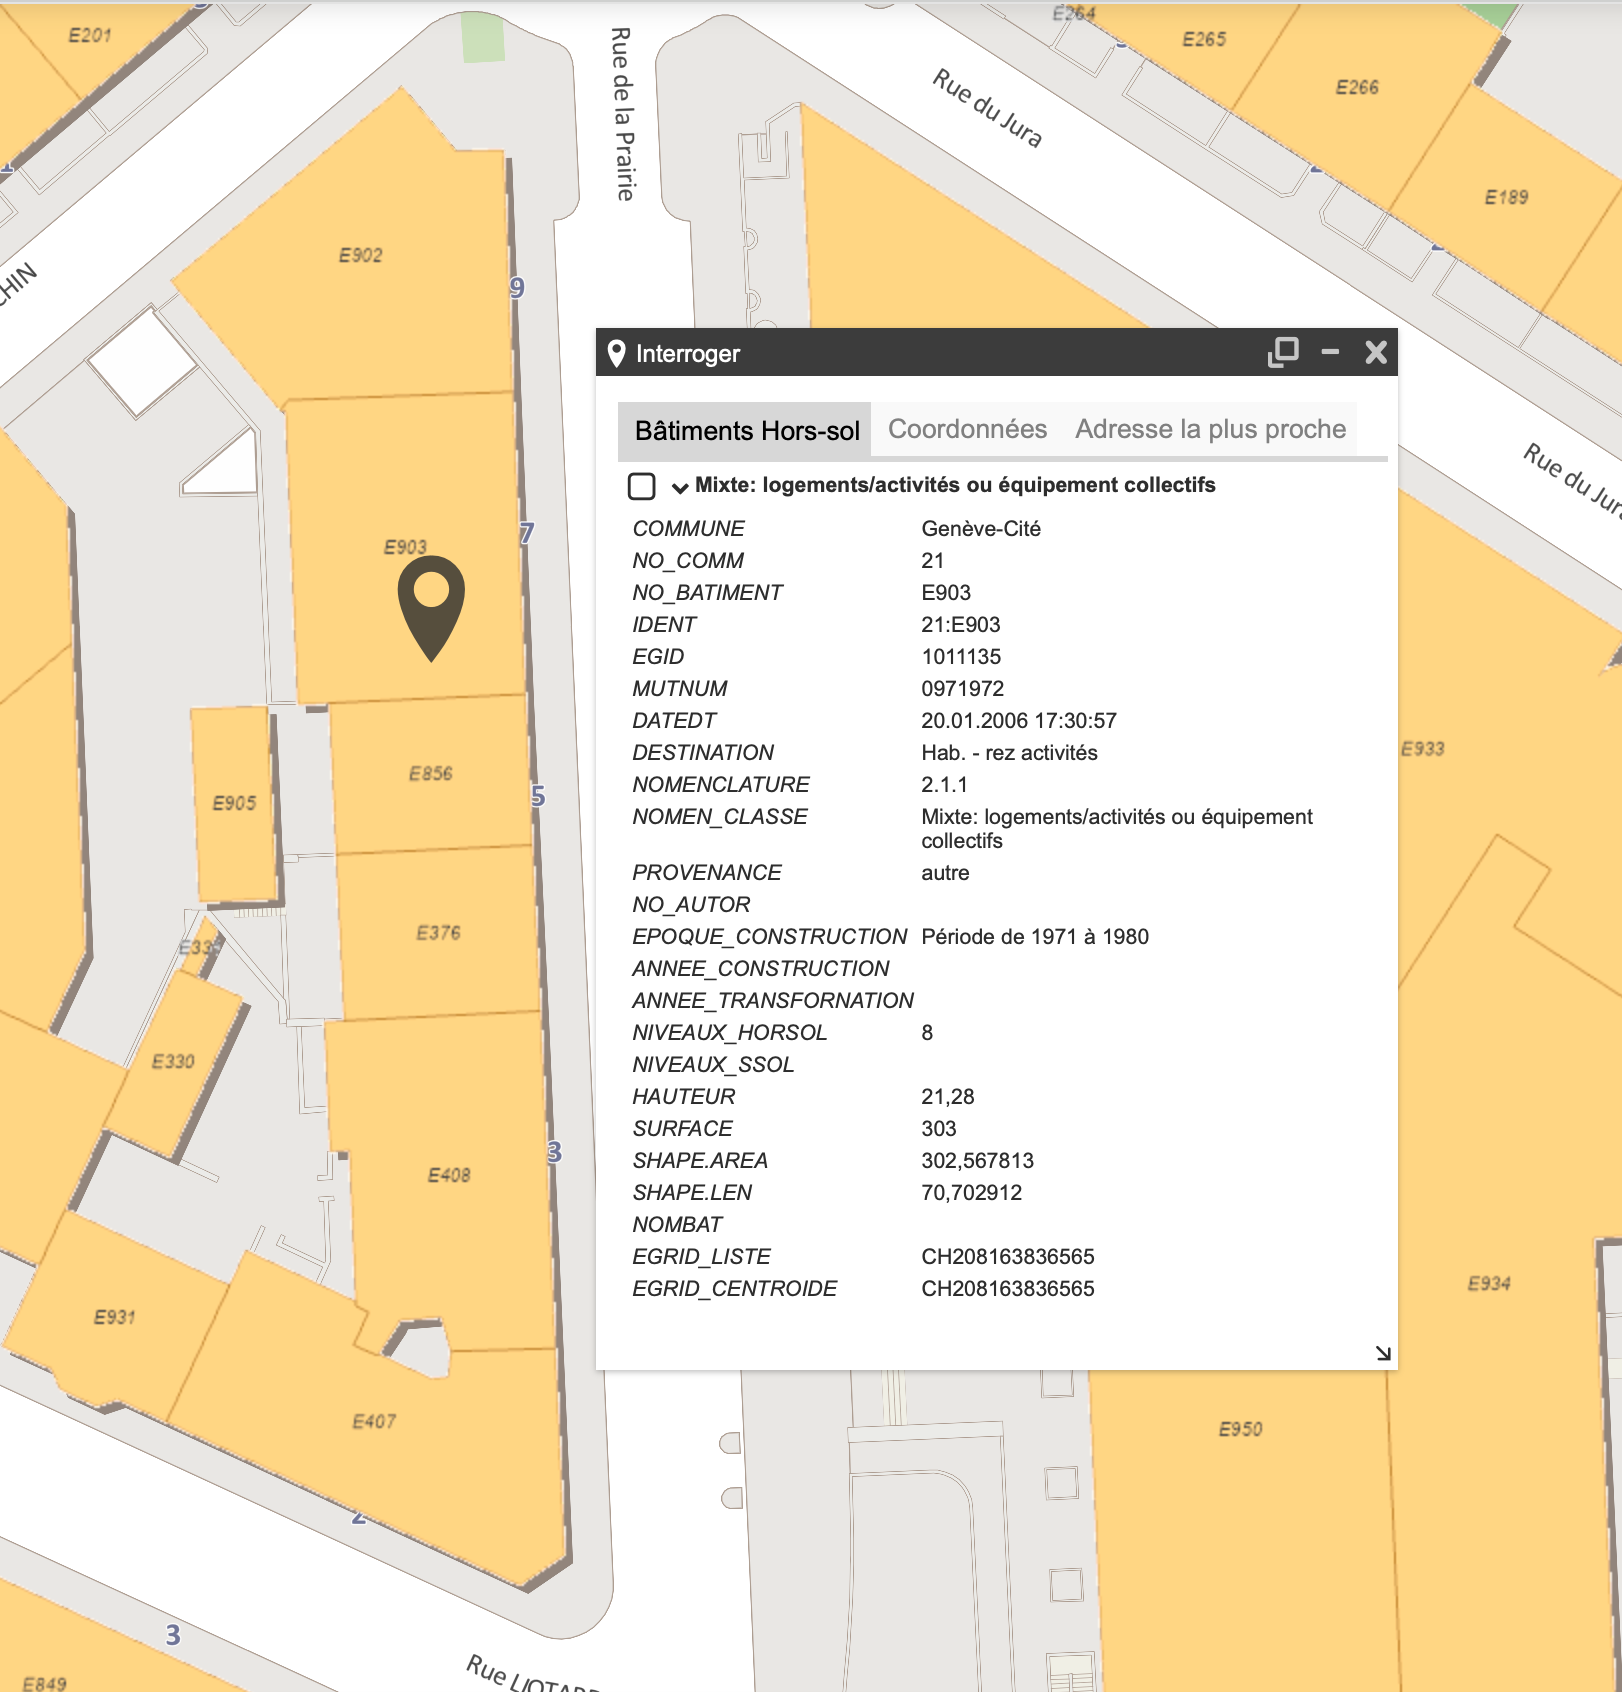
\includegraphics[width=1\linewidth]{02-main//figures/dataset_methodo_02_batiment_horsol_donnees.png}
    \caption{Exemple de données tabulaire associée a un bâtiment (polygone)}
    \label{fig:dataset_methodo_02_batiment_horsol_donnees}
\end{figure}
Les données intéressantes sont l'``EGID'' et ``NOMEN\_CLASSE''. L'EGID est un identifiant unique pour tous les bâtiments en Suisse


% -----------------------------------------------------------------------------
% -----------------------------------------------------------------------------
\section{Pistes explorées non retenues}
\subsection{Introduction}
Cette section va permettre de synthétiser les approches essayées mais qui n'ont pas été retenues. Ce travail exploratoire est nécessaire mais il peut être difficile à valoriser à sa juste valeur.

La première sous-section va explorer la classification des données des toitures et l'utilisation de segment anything model, ensuite la deuxième va explorer les possibilités d'utilisation du dataset RID.

\subsection{Classification}
\subsubsection{Hypothèse}
\acrshort{sitg} met à disposition des données concernant les toitures mais aussi les superstructures présentes sur ces toitures. Une approche naïve serait d'estimer que les toitures qui ne disposent d'aucune superstructure dans leur toiture sont a priori libres. Les toitures restantes avec une superstructures sont ensuite segmentées à l'aide de segment anything model (SAM).

\subsubsection{Données}
Les données utilisées proviennent de \acrshort{sitg}:
\begin{itemize}
    \item Emprise des toitures au sol ``CAD\_BATIMENTS\_HORSOL\_TOIT'' \cite{sitg_toits_nodate}
    \item Superstructures des toits des bâtiments ``CAD\_BATIMENT\_HORSOL\_TOIT\_SP'' \cite{sitg_superstructures_nodate}
    \item Pourcentage des besoins de chauffage couverts
\end{itemize}







